\documentclass{codedoc}

\usepackage{lmodern,tikz,graphicx,shortvrb,url,xspace}
\usepackage[small]{titlesec}
\usepackage[margin=1in]{geometry}

\MakeShortVerb{\|}
\newcommand{\option}[3]{\item [\texttt{#1}] (\meta{#2}; default: \texttt{#3}).}
\newcommand*{\pkgname}{\texttt{pdfreview}\xspace}

\author{Michael Palmer}
\title{The \pkgname package}
\date{v1.00 (\today)}

\usepackage{bookmark}

\begin{document}

\maketitle

\begin{abstract}
\noindent The \pkgname package lets you add comments in the page margins of PDF files, e.g.\ when reviewing manuscripts or grading reports. The PDF file to be annotated is included, one page at a time, as graphics, in a manner similar to the \texttt{pdfpages} package. Notes are placed in the margin next to the included graphics using a grid of help lines. Alternatively, only numbers are placed in the page margins, and the notes are collected into a numbered list at the end of the document. \par
Note that this package is \emph{not} intended for adding notes directly to the \LaTeX{} source of the document that is being reviewed; instead, the document undergoing review is already in PDF format and remains unchanged. Also note that this package does not produce the usual PDF `sticky notes' that must be opened by clicking on them; instead, the notes are simply shown as text. 
\end{abstract}

\section{An example}

Let's assume a student submitted his essay as \texttt{lorem-ipsum.pdf}. In order to review and annotate it, I create this wrapper \LaTeX{} document:

\begin{verbatim}
\documentclass[letterpaper,10pt]{article}

\usepackage[
  sourcedoc=lorem-ipsum.pdf,      % declare the PDF document being reviewed
  grid=true,                      % draw help lines for margin notes (set false when done)
  bodywidth=0.66,                 % set width of source doc page as fraction of \textwidth
  twocolumn=true,                 % place margin notes on both sides
  trim=2cm,                       % trim all page margins of source doc by this amount
]{pdfreview}

\begin{document}

\begin{page}{1}                   % mount the first page

\begin{leftnotes}                 % write notes into the left margin
\cnote{84}{It looks like Latin.}  % place note centered on help line 84
\bnote{68}{Is this really Latin?} % align bottom of note to help line 68
\tnote{16}{No, not Latin}         % align top of note to help line 16
\end{leftnotes}                   % notes after this point go into the right margin

\tnote{48}{You really should be writing proper Latin}
\cnote{12}{Cite your references}
\end{page}

% \begin{page}{2}                 % mount the next page
% \note{...}{...} etc.

\end{document}
\end{verbatim}
\clearpage 

\noindent This gives us the following output (only the first page is shown):

\begin{center}
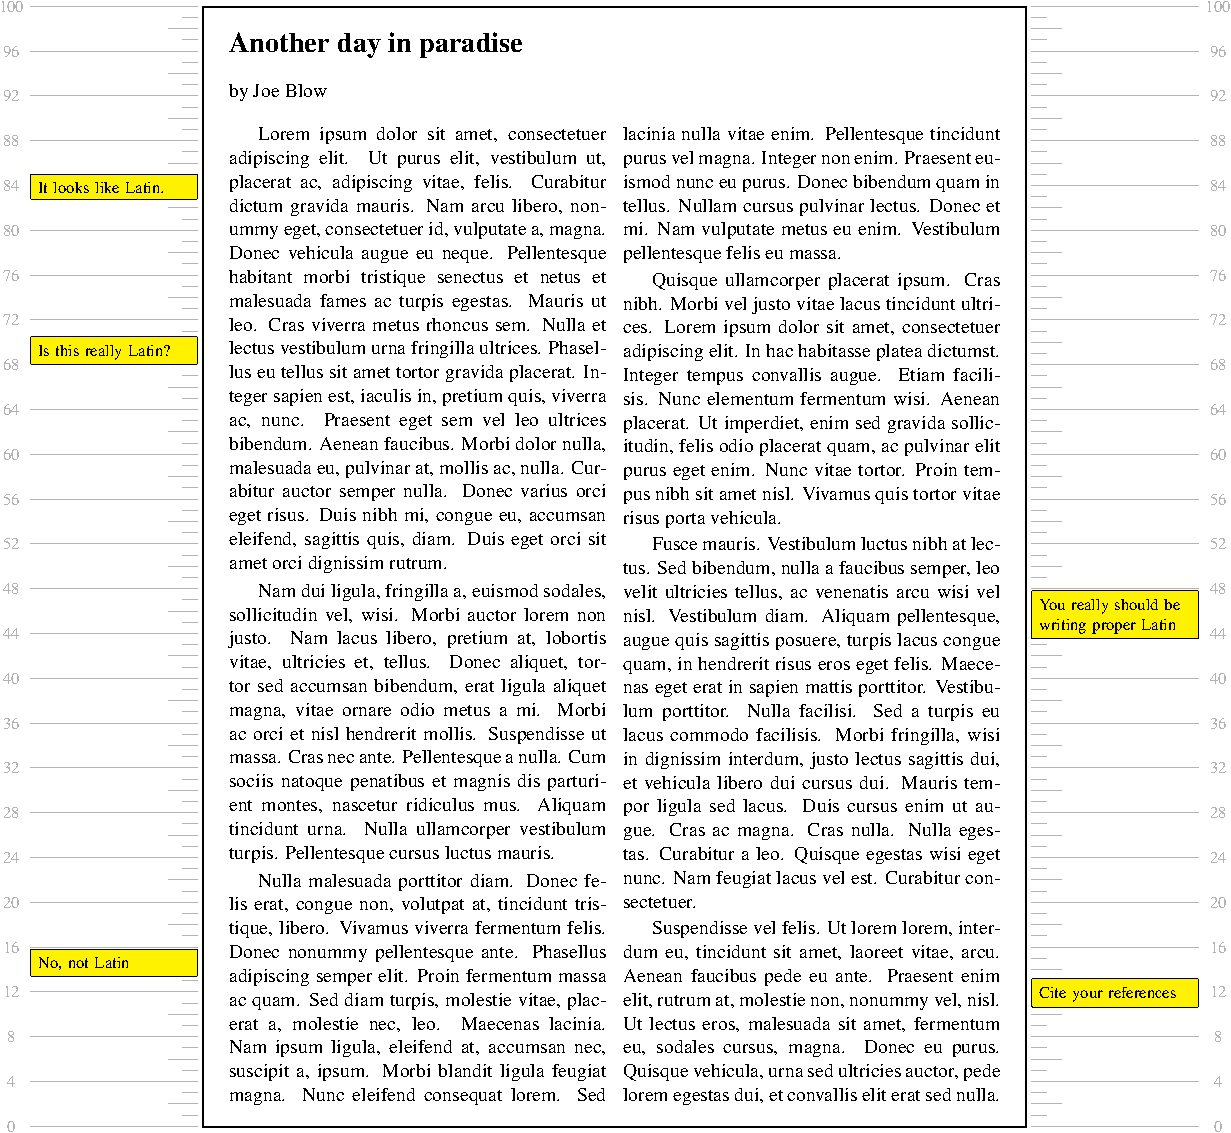
\includegraphics[width=\textwidth]{sample-for-docs}
\end{center}

When you have added all your comments, you can set the package option \texttt{grid=false} in order to hide the help lines. That is essentially it, already; some more options and a few tips and tricks will be given below. 

\section{Package options}

\begin{description}

\option{sourcedoc}{file name}{noname} Name of the PDF file to be reviewed. The file extension (\texttt{.pdf}) can be omitted. 

\option{twocolumn}{boolean}{false} If true, place included page in the middle and arrange for margin notes on both sides. If false, place included page on the left and have margin notes on the right hand side only. 

\option{inline}{boolean}{true} If true, print the note text into the page margin. If false, print only the number of each note into the page margin. In the latter case, the note text will be collected and printed out as an \texttt{enumerate}'d list at the end of the document. Numbers in the margin and list items will be reciprocally hyperlinked.

\option{notenumbers}{boolean}{false} If true, start each note with its number. If option \texttt{inline} is false, the number is printed regardless of this option. 

\option{grid}{boolean}{true} Draw help lines for margin notes. 

\option{gridcolor}{color name}{black!30} Color to use for help lines and line numbers. 

\option{maxscale}{number}{100} Number of vertical length units/help lines for placing margin notes. If not divisible by 4, you will get a few ugly surplus lines at the top. 

\option{stretch}{number}{1} By default, the vertical scale for placing margin notes is exactly as high as the first source document page. If that doesn't work well for some reason---for example, because you manually trim some pages more than others (see below)---then you can use this fudge factor to adjust the height of the scale manually. The scale will always be the same for all pages though.   

\option{bodywidth}{number}{0.75} Width of the included source doc page, as fraction of \texttt{\textbackslash textwidth} of the wrapper document. The remainder of \texttt{\textbackslash textwidth} will be used for the margin notes. 

The default of 0.75 should be suitable in combination with \texttt{inline=true,twocolumn=false}, that is, with full note text in the right margin only (which is my own most common use case). Use smaller values with \texttt{inline=true,twocolumn=true} or larger ones with \texttt{inline=false}. 

\option{trim}{length(s)}{1cm} How much to trim off the margins of each page of the source document. This option is passed to the \texttt{\textbackslash adjustbox} macro from the package by the same name. Accordingly, you can use two lengths to specify separate trimmings for horizontal and vertical margins, and four lengths to specify separate values for the left, lower, right, and top margins (in this order. No, it doesn't resemble a clock, fuel gauge, or anything else that mere mortals might have encountered). 

Note that multiple lengths values must be surrounded with braces, e.g.\ \texttt{trim=\textbraceleft 1cm 2cm\textbraceright} or \texttt{trim=\textbraceleft 1cm 2cm 0cm 1cm\textbraceright}. If you omit the braces, only the first length value will be used, and the others will be silently ignored. 

\option{alignnotes}{t,b, or c}{c} Vertical alignment of a margin note declared with |\note|. Can be overridden by passing \texttt{t} or \texttt{b} as an optional argument (e.g.~|\note[b]{Go boil your bottoms}| or |\note[t]{I shall taunt you a second time}|). 

\option{notesbg}{color name or `none'}{yellow} Background color to use for the margin notes. If `none', the background will be transparent. 

\option{notesframe}{color name or `none'}{black} Color to use for the box frame of the margin notes. If `none', no box is drawn. 

\option{notesep}{length}{3pt} Empty space between included page and margin notes.

\option{fontsize}{string}{footnotesize} Font size to use for the margin notes. Use any of the usual font size commands, but without the backslash.

\option{pageoffset}{number}{0} This option only affects the PDF bookmarks for each page of the current document; it is intended to synchronize the bookmarks with the page numbers of the source document. 

By default, \pkgname simply numbers all included pages consecutively, starting with 1. If the source document has, say, 5 unnumbered (or Roman-numbered) pages preceding the proper page 1, you can declare this with \texttt{pageoffset=-5}; in this case, the first 5 pages will be given Roman numerals, and Arabic numbers will start (at 1) on the sixth physical page. Similarly, if the source document is missing some logical pages at the beginning, you can correct for this using a positive value for \texttt{pageoffset}.

(As usual, the least useful options require the most explanation.)

\option{insertpagemargin}{length}{2.5cm} If you have comments of a general nature, or ones that don't fit comfortably into the page margin, you can put them on separate pages insert one or more empty pages using the \texttt{insertpage} environment (see below).

By default, \pkgname leaves only very narrow empty page margins beyond the margin notes. For inserted text pages, it is more appropriate to use a wider margin; you can adjust it with this option. 

\end{description}

\section{Macros}

\begin{description}

\item [{\texttt{\textbackslash note[\meta{alignment}]\marg{height}\marg{text}}}] 
      The optional \texttt{alignment} argument is one of \texttt{b}, \texttt{c}, or \texttt{t}. The \meta{height} argument names the help line to align to; \meta{text} is the content of the note. (The \meta{height} argument doesn't have to be an integral number. Also, it can fall outside of the displayed help line scale, within reason.)
      
      Note that the entire text of each note will go inside a \texttt{TikZ} node. This means you cannot use empty lines within a note to insert paragraphs. If you do need paragraphs, use the |\par| macro instead.
      
\item [\texttt{\textbackslash bnote}\marg{height}\marg{text}] 
      Shorthand for \texttt{\textbackslash note[b]\marg{height}\marg{text}}. Analogous |\cnote| and |\tnote|. 

\item [\texttt{\textbackslash sourcedoc}\marg{file name}] Set the file name of the PDF file whose pages are to be included. More commonly, this is done using the \texttt{sourcedoc} package option (see above). However, this macro can be used to switch to another source document halfway through. 

\end{description}

\section{Environments}

\begin{description}

\item [\texttt{\textbackslash begin\textbraceleft page\textbraceright [\meta{graphics options}]\marg{page number} \ldots\ \textbackslash end\textbraceleft page\textbraceright}] 

This environment loads the physical page \meta{page number} from the source document and sets up the container for the margin notes. The formatting and scaling of the included page and of the margin notes is subject to the package options described earlier. 

The optional \meta{graphics options} are passed to the \texttt{\textbackslash adjustbox} macro from the  package of the same name. You could use this for example to override the global \texttt{trim} package option for this one page, like so: \texttt{trim=0cm 1cm}. 

\item [\texttt{\textbackslash begin\textbraceleft leftnotes\textbraceright \ldots\ \textbackslash end\textbraceleft leftnotes\textbraceright}] 

This environment goes inside a \texttt{page} environment. In \texttt{twocolumn} mode, it will move the enclosed |\note| macros to the left page margin; with \texttt{twocolumn=false} it does nothing, that is, notes enclosed in \texttt{leftnotes} will show up in the right margin. 

\item [\texttt{\textbackslash begin\textbraceleft rightnotes\textbraceright \ldots\ \textbackslash end\textbraceleft rightnotes\textbraceright}] Never does anything, ever; it only exists to avoid tripping up users who surmise its existence from that of the \texttt{leftnotes} environment. 

\item [\texttt{\textbackslash begin\textbraceleft insertpage\textbraceright [\meta{heading}] \ldots\ \textbackslash end\textbraceleft insertpage\textbraceright}] 

Inserts one or more extra pages for longer comments. These are not subject to any special formatting, except for the page margin, which can be set using a package option (see above). Alternatively, you can set the margins manually using |\newgeometry| and |\restoregeometry| from the \texttt{geometry} package, which is loaded by \pkgname. (The optional argument \meta{heading} defaults to ``General comments''.)

\end{description}

\section{Practical recommendations}

\subsection{Page space usage}

Obviously, one needs to make some judicious choices in order to allow enough space for our margin comments yet also keep the included PDF pages legible. Use the \texttt{trim} package option to shave off empty margins from the included PDF pages. 

The \texttt{geometry} package will be loaded to divide up the page. By default, \pkgname leaves 0.25 cm empty margins on both sides. If you load the \texttt{geometry} package yourself, \pkgname will respect your settings and not impose its own margin width. In that case, note that the entire content---included PDF page and margin notes---will go inside |\textwidth|. Any margins you declare using the \texttt{geometry} package will remain entirely empty. Also note that any \texttt{geometry} settings can be declared in the preamble only; if you try to change the margins within the document using |\newgeometry|, things will unravel. 

\subsection{Vertical overlap of margin notes}

There is no automatic mechanism that would prevent mutual overlap of margin notes; this has to be prevented manually. Where space is tight, it may help to use e.g.\ a |\tnote{60}{some note}| followed by a |\bnote{60}{another note}|; no space is wasted between both notes, yet at the same time they will not overlap. 

The \texttt{bodywidth} package option also decides the horizontal and vertical space available for the margin notes. Should you decide half-way through to reduce the \texttt{bodywidth} parameter, this will create more horizontal space for the notes, but at the same time reduce the vertical space. This may occasionally create some new vertical overlap that would have to be fixed manually.

Another consideration is what font to use for your notes, and at what size. Times is a nice, space-saving font (in pdfLaTeX, you can load with |\usepackage{mathptmx}|). You can adjust the font size using the corresponding package option (e.g.~\texttt{fontsize=scriptsize}).

\subsection{Writing less boiler plate code}

While the code to set up each page is pretty compact, it can still become tiresome to write for long source documents. The package includes a \texttt{bash} script named \texttt{pdfreview.sh}, which generates a document skeleton containing a \texttt{page} environment for each page of a source document: 

\begin{verbatim}
mpalmer@holzkopf:/data$ pdfreview.sh source.pdf > review.tex
\end{verbatim}

\noindent The script requires 1) \texttt{ghostscript}, 2) \texttt{bash} (obviously) and 3) that you place it somewhere into your shell's path. 

\subsection{File size}

Particularly when working with large source files, \pkgname can produce some startlingly large PDF output files. This problem is apparently related to the way |\includegraphics| works and has been described before (see \url{https://tex.stackexchange.com/questions/207527/}).
%
It can be amended by post-processing the output PDF file with ghostscript, for example: 

\begin{verbatim}
gs -sDEVICE=pdfwrite -dCompatibilityLevel=1.4 -dPDFSETTINGS=/printer -dNOPAUSE -dQUIET \
   -dBATCH -sOutputFile=post-processed.pdf output.pdf
\end{verbatim}

\noindent The package contains a bash script named \texttt{pdfshrink.sh} that wraps the call to \texttt{ghostscript} and which you can use like 

\begin{verbatim}
mpalmer@holzkopf:/data$ pdfshrink.sh large.pdf small.pdf 
\end{verbatim}

\noindent Again, you need to save the script in a directory listed in your shell's search path for this work. 

\subsection{Uncooperative input files}

Occasionally, I've run into source documents that failed to cooperate with the page-wise inclusion attempted by \pkgname. I got around that by first printing the recalcitrant PDF input file to another PDF file---or, alternatively, run through \texttt{pdfshrink}---and then using the resulting file as the source document instead. (This might also be useful on occasion when using the \texttt{pdfpages} package.)

\section{Implementation}

This package depends on several other ones that are all in TeXLive. Among these is the \texttt{ulem} package, which makes the |\sout{strike me out}| command available for a strike-through effect (see first note in the above example). The \texttt{geometry} package is used for dividing up the page; if you load it yourself, your settings will be respected, as long you declare them in the preamble (but don't use |\newgeometry| halfway through the document). The \texttt{adjustbox} package is used to scale and trim the included pages, and also to scale the containers for the margin notes. The \texttt{tikz} package is used for placing help lines and margin notes. 
      
For further details, see the package file itself.

\section{Revision history}

May 2017: initial version (1.00)

\section{License}

All files in this package are subject to the LaTeX project public license (see \url{http://www.latex-project.org/lppl.txt}). 


\end{document}